
%(BEGIN_QUESTION)
% Copyright 2013, Tony R. Kuphaldt, released under the Creative Commons Attribution License (v 1.0)
% This means you may do almost anything with this work of mine, so long as you give me proper credit

Examine the main fractionator level control system (at the bottom of the fractionator tower) and explain why three different types of level transmitter are used:

$$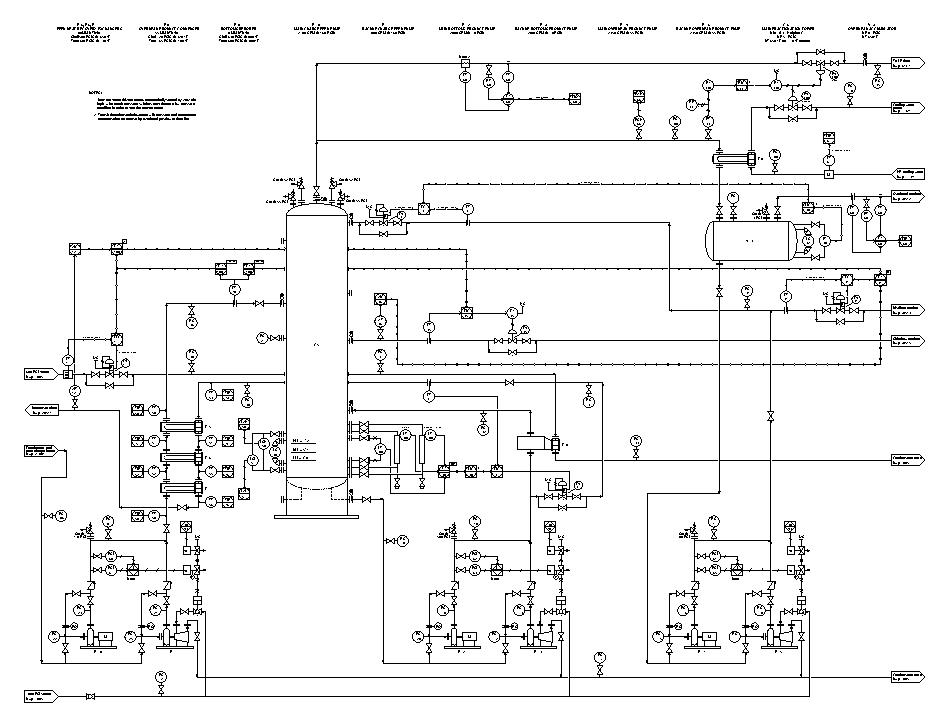
\includegraphics[width=15.5cm]{i0001rx02.eps}$$

Also, if you have studied level transmitter technologies, identify how we might change {\it one} of those level transmitter types to achieve better reliability.  As it stands right now, two of those transmitters may be ``fooled'' by one change in process liquid characteristics, which means there exists the potential for a ``common-cause'' failure in this measurement system.

\underbar{file i03364}
%(END_QUESTION)





%(BEGIN_ANSWER)

The three level transmitters (LT-38a, LT-38b, and LT-38c) are supposed to be {\it redundant} to each other: all sensing the exact same liquid level inside the fractionator tower, but using different technologies.  The selector function used between these three transmitters is a {\it median-select}, choosing the middle value of the three.  This essentially functions as a ``best-2-out-of-3'' selector because if any one transmitter gives a reading significantly different from the other two it will be de-selected by LY-38.
 
\vskip 10pt

The problem with the instrument choices in this application is that of the differential pressure (DP) based transmitter LT-38a and the displacer (buoyancy) based transmitter LT-38b.  Both of these instruments' calibrations are affected in the exact same way by changes in liquid density.  Therefore, if the density of the liquid in the bottom of the fractionator tower were to change significantly for some reason, as can happen during start-up, shut-down, or ``upset'' conditions, those two transmitters will output the same erroneous results.  With two out of the three transmitters agreeing with each other, the selector function LY-38 will choose the wrong level measurement signal and reject the signal given by the float-type transmitter LT-38c even though that transmitter will not be affected by the change in liquid density and will be reporting the correct level value.

%(END_ANSWER)





%(BEGIN_NOTES)

\filbreak \vskip 20pt \vbox{\hrule \hbox{\strut \vrule{} {\bf Virtual Troubleshooting} \vrule} \hrule}

\noindent
{\bf Predicting the effect of a given fault:} present each of the following faults to the students, one at a time, having them comment on all the effects each fault would produce.

\begin{itemize}
\item{} FT-40 fails low
\item{} FT-35 fails high
\item{} LT-38a fails low
\item{} LT-38a fails high
\item{} Loss of instrument air to FV-37
\item{} PSL-60 fails low
\end{itemize}


\vskip 10pt


\noindent
{\bf Identifying possible/impossible faults:} present symptoms to the students and then have them determine whether or not a series of suggested faults could account for all the symptoms, explaining {\it why} or {\it why not} for each proposed fault:

\begin{itemize}
\item{} Symptom: {\it }
\item{}  -- {\bf Yes/No}
\item{}  -- {\bf Yes/No}
\item{}  -- {\bf Yes/No}
\end{itemize}


\vskip 10pt


\noindent
{\bf Determining the utility of given diagnostic tests:} present symptoms to the students and then propose the following diagnostic tests one by one.  Students rate the value of each test, determining whether or not it would give useful information (i.e. tell us something we don't already know).  Students determine what different results for each test would indicate about the fault, if anything:

\begin{itemize}
\item{} Symptom: {\it }
\item{}  -- {\bf Yes/No}
\item{}  -- {\bf Yes/No}
\end{itemize}


\vskip 10pt


\noindent
{\bf Diagnosing a fault based on given symptoms:} imagine the ??? fails ??? in this system (don't reveal the fault to students!).  Present the operator's observation(s) to the students, have them consider possible faults and diagnostic strategies, and then tell them the results of tests they propose based on the following symptoms, until they have properly identified the nature and location of the fault:

\begin{itemize}
\item{} Operator observation: {\it }
\item{} 
\item{} 
\end{itemize}
%INDEX% Process: distillation, generic (realistic P&ID shown)

%(END_NOTES)


